\section{Error Locator}
\label{sec:error_locator}

Differential fuzzing can determine whether a target \zksnark program produces a result that is inconsistent with the statement-level oracle. However, this result alone does not tell developers where the error occurs. A mismatch may be caused by an incorrect circuit, an incorrect witness conversion, an error in proof generation, or an error in proof verification. This problem is more difficult in the binary-only setting because \greyboxfuzz does not rely on source-level annotations, source-code structure, or manually inserted debugging information.

To provide more useful feedback, \greyboxfuzz includes an error locator that identifies the component most likely responsible for a detected inconsistency. Given a seed that triggers a mismatch, the error locator distinguishes among five possible sources: the circuit, the prover-side input converter, the core proving function \pfunc, the verifier-side public-input converter, and the core verification function \vfunc. This component-level feedback reduces the amount of manual debugging required after fuzzing discovers a security vulnerability or \logicerror.

\begin{figure}[t]
  \centering
  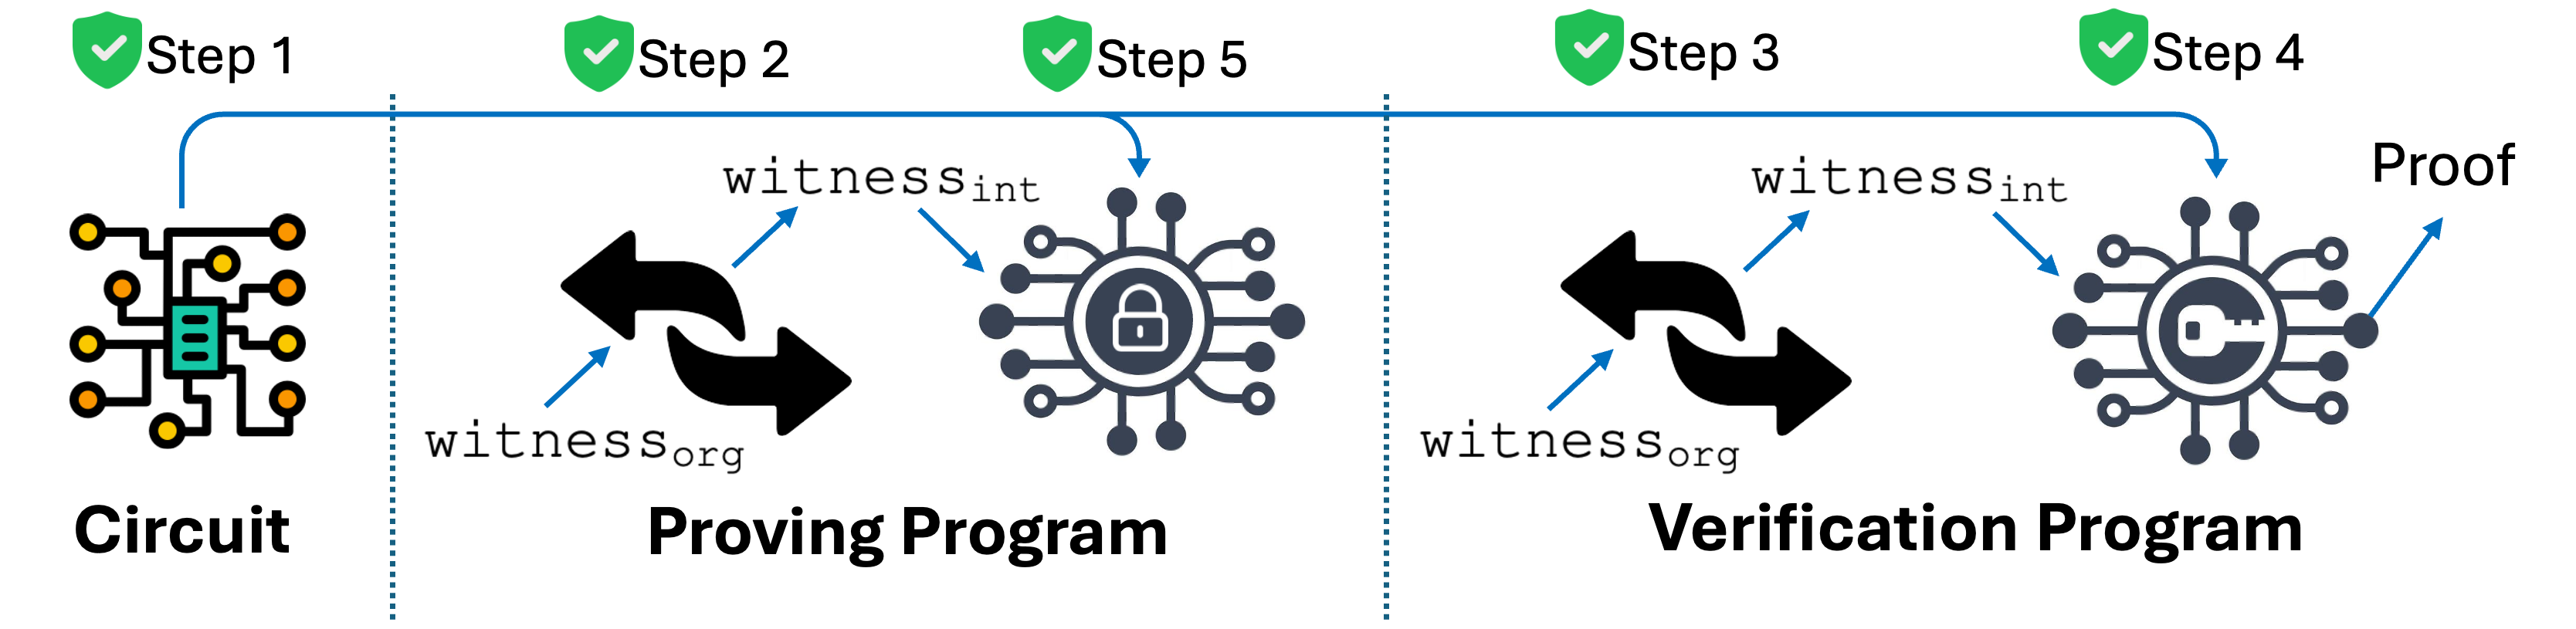
\includegraphics[width=\columnwidth,keepaspectratio]{./ch-greybox/figure/error_locator.png}
  \caption{Error localization procedure in \greyboxfuzz.}
  \label{fig:error_locator}
\end{figure}

\subsection{Error Model}

As discussed in \autoref{subsec:structure_zkp}, a \zksnark application contains two complete programs: the prover-side program \pprog and the verifier-side program \vprog. The prover-side program parses the original witness \witnessorg, converts it into the internal witness representation \witnessint, and invokes \pfunc to generate a proof. The verifier-side program parses the proof and public input, converts the public input into the internal representation expected by the verifier, and invokes \vfunc to output an accept or reject result.

The circuit itself may also be incorrect. The circuit defines the arithmetic constraints that the proof system enforces. If the circuit does not correctly represent the intended statement, then even a correct prover and verifier may produce a result that disagrees with the statement-level oracle. Therefore, \greyboxfuzz considers five possible error locations:

\begin{itemize}[leftmargin=*]
    \setlength{\itemsep}{0pt}
    \setlength{\parskip}{0pt}
    \item the circuit that encodes the intended statement;
    \item the prover-side input converter that transforms \witnessorg into \witnessint;
    \item the core proving function \pfunc;
    \item the verifier-side public-input converter;
    \item the core verification function \vfunc.
\end{itemize}

The goal of the error locator is not to prove the global correctness of all components. Instead, for a seed that already exposes an inconsistency, the error locator performs a sequence of checks to identify the first component that can explain the mismatch.

\subsection{Identifying Prover and Verifier Components}

Before \greyboxfuzz can localize an error, it must identify the component boundaries inside \pprog and \vprog. Since \greyboxfuzz targets binary programs, this step cannot rely on source-code annotations.

If the target programs dynamically link against a \zksnark library, such as \libsnark or \bellman, \greyboxfuzz can identify \pfunc and \vfunc through imported symbols, dynamic-library calls, and argument patterns. In this case, the call boundary between application code and cryptographic library code provides a natural point for extracting intermediate values.

If the target programs statically link the \zksnark library, the proving and verification functions are compiled into the same binary as the surrounding application logic. In this case, \greyboxfuzz uses the static taint tracking technique described in \autoref{subsec:branch_identify} to infer the locations of \pfunc and \vfunc.

For \pprog, \greyboxfuzz treats the circuit, \witnessorg, and proving key as taint sources. The prover-side input converter transforms \witnessorg into \witnessint, and \pfunc consumes \witnessint together with the circuit and proving key to produce a proof. Therefore, \greyboxfuzz identifies \pfunc by searching for a function that satisfies the following conditions:

\begin{itemize}[leftmargin=*]
    \setlength{\itemsep}{0pt}
    \setlength{\parskip}{0pt}
    \item It receives the circuit or circuit-derived data;
    \item It receives the proving key;
    \item It receives \witnessint, which is tainted from \witnessorg;
    \item It produces a proof object or proof-derived output.
\end{itemize}

For \vprog, \greyboxfuzz treats the proof, public input, and verification key as taint sources. The verifier-side public-input converter transforms the public input into the internal representation required by \vfunc. Then, \vfunc checks the proof using the verification key and the converted public input. Therefore, \greyboxfuzz identifies \vfunc by searching for a function that satisfies the following conditions:

\begin{itemize}[leftmargin=*]
    \setlength{\itemsep}{0pt}
    \setlength{\parskip}{0pt}
    \item It receives the verification key;
    \item It receives the proof;
    \item It receives the internal representation of the public input;
    \item It returns the accept or reject result.
\end{itemize}

After identifying these component boundaries, \greyboxfuzz hooks the corresponding program locations and extracts the intermediate values required for localization.

\subsection{Localization Procedure}

The error locator is invoked only after differential fuzzing detects a mismatch. For each generated seed, \greyboxfuzz first evaluates the intended statement using the Charm-based oracle described in \autoref{sec:differential}. It then executes the target \pprog and \vprog and compares the target verification result with the oracle result. If the two results match, the seed does not trigger localization. If the two results differ, \greyboxfuzz applies the sequential localization procedure shown in \autoref{fig:error_locator}.

The procedure checks possible error sources in the following order:

\begin{itemize}[leftmargin=*]
    \setlength{\itemsep}{0pt}
    \setlength{\parskip}{0pt}
    \item \textbf{Step 1}: Check whether the circuit correctly represents the intended statement.
    \item \textbf{Step 2}: Evaluate the circuit using the prover-side internal witness.
    \item \textbf{Step 3}: Compare the prover-side and verifier-side representations of public inputs.
    \item \textbf{Step 4}: Compare \vfunc with an independent verification implementation.
    \item \textbf{Step 5}: If all previous checks pass, attribute the remaining inconsistency to \pfunc.
\end{itemize}

This order is important. The circuit is checked first because an incorrect circuit can make all later components appear inconsistent with the intended statement. The prover-side witness conversion is checked next because \pfunc depends on the converted witness. The verifier-side public-input conversion is then checked because the verifier may interpret the public input differently from the prover. Finally, \vfunc is checked against an independent verifier. If none of these components explains the mismatch, the remaining likely source is \pfunc.

\subsection{Step 1: Circuit Validation}
\label{subsec:locate_circuit}

The first step checks whether the circuit correctly encodes the intended statement. A circuit is the constraint representation used by the proof system. It defines the arithmetic relations that must be satisfied for a proof to be valid. If the circuit is under-constrained, over-constrained, or inconsistent with the intended statement, then the program may produce proofs that are valid for the circuit but invalid for the statement the developer intended to enforce.

When existing circuit-analysis tools are applicable, \greyboxfuzz uses them to check the circuit against the intended statement. For example, tools such as Picus and ConstraintChecker can help identify circuit-level problems, including missing constraints or inconsistencies between the circuit and the expected computation. If this check shows that the circuit does not correctly represent the statement, \greyboxfuzz attributes the mismatch to the circuit rather than to \pprog or \vprog.

\subsection{Step 2: Prover-Side Witness Conversion}

If the circuit passes validation, \greyboxfuzz checks whether the prover-side input converter correctly transforms \witnessorg into the internal witness representation for the current seed. In a \zksnark program, the original witness may be represented as application-level values, such as integers, byte strings, group elements, or encoded objects. Before proof generation, these values must be converted into the representation expected by the circuit, typically finite-field elements.

\greyboxfuzz hooks \pprog after the prover-side conversion step and extracts the internal witness. It then evaluates the circuit directly using this extracted witness. If the circuit evaluation result differs from the Charm oracle result, then the extracted witness does not correctly represent the original input with respect to the intended statement. Since Step~1 has already checked the circuit, this mismatch indicates that the prover-side input converter produced an incorrect internal witness for the current seed.

This step localizes errors such as incorrect parsing, wrong field encoding, missing range conversion, endian mismatch, sign-handling errors, or inconsistent mapping from application-level values to field elements.

\subsection{Step 3: Verifier-Side Public-Input Conversion}

The verifier does not receive the prover's private witness. Therefore, \greyboxfuzz does not compare the full private witness representation between \pprog and \vprog. Instead, this step checks the public inputs, which are used by both the prover and verifier.

The prover and verifier may be developed by different parties or built using different libraries. Even if the prover-side conversion is correct for the current seed, the verifier-side converter may parse or encode the same public input differently. In that case, the verifier may check the proof against a different internal public input from the one used during proof generation.

To detect this class of error, \greyboxfuzz extracts the prover-side internal representation of the public inputs and compares it with the verifier-side internal representation of the same public inputs. If the two representations differ, \greyboxfuzz attributes the mismatch to the verifier-side public-input converter. This indicates that \vprog failed to convert the public input into the representation expected by \vfunc.

This step localizes errors such as inconsistent public-input encoding, different field-element serialization, incorrect modulus handling, and parsing differences between prover-side and verifier-side programs.

\subsection{Step 4: Verification Function Checking}

If the circuit and input converters are consistent, \greyboxfuzz checks the core verification function \vfunc. This step determines whether the verifier's cryptographic computation produces the correct accept or reject result for the proof, public input, and verification key.

The verification function in a \zksnark protocol is much simpler than the proving function. While proof generation depends on the witness, circuit, proving key, and protocol-specific randomness, proof verification mainly consists of elliptic-curve operations, scalar operations, and pairing checks over the verification key, public input, and proof. This structure makes the verifier a practical target for independent reimplementation.

A straightforward way to build this independent verifier is to use a trusted cryptographic library such as \texttt{py\_ecc}. Given the proof, verification key, and converted public input, the \texttt{py\_ecc}-based verifier recomputes the expected pairing equation and returns an accept or reject result. \greyboxfuzz then compares this result with the output of \vfunc in the target binary. If the two results differ, the inconsistency indicates that the verifier implementation in the target binary may be incorrect. This approach is useful because it avoids the need to reimplement the entire \zksnark system. It only requires an independent implementation of the verification equation for the selected curve and proof system.

However, an implementation based on a standard cryptographic library still relies on the correctness of that library and of our verifier implementation. To provide stronger confidence, \greyboxfuzz can replace the \texttt{py\_ecc}-based verifier with a formally verified verifier when the required curve and operations are supported. We build this verified verifier using HACL*, a formally verified cryptographic library developed as part of the Project Everest \cite{zinzindohoue2017hacl, project_everest}. HACL* is implemented in F* and provides verified implementations of cryptographic primitives, including elliptic-curve operations~\cite{zinzindohoue2016verified}. By building the verifier on top of verified cryptographic components, \greyboxfuzz obtains a higher-assurance reference implementation for checking \vfunc.

The formally verified verifier does not attempt to verify the entire \zksnark application or the full proving algorithm. Instead, it focuses on the verification computation, which is the part of the protocol used by \greyboxfuzz to distinguish verifier-side errors from prover-side errors. For a given proof instance, the verified verifier checks that the pairing equation and related elliptic-curve computations are performed according to the expected verification algorithm. The output of this verified implementation is then used as the reference result for \vfunc. If the target binary verifier disagrees with the verified verifier, \greyboxfuzz attributes the inconsistency to the verification function.

This design has two benefits. First, it provides a practical verifier oracle that can be used even when source code is unavailable. Second, when the HACL*-based backend is available, the oracle has stronger assurance than a conventional library-based implementation because the underlying cryptographic operations are formally verified. This improves the reliability of the error locator: a mismatch between \vfunc and the verified verifier is less likely to be caused by an error in the oracle itself.

The current limitation is curve and protocol support. A verified verifier must be implemented for the specific elliptic curve and verification equation used by the target \zksnark program. HACL* supports only a limited set of elliptic-curve operations, so not every target can use the formally verified backend. When the required curve or pairing operation is not supported, \greyboxfuzz falls back to the \texttt{py\_ecc}-based verifier. Although this fallback provides lower assurance than the formally verified implementation, it still offers an independent reference for localizing errors in \vfunc. Expanding the verified backend to support more curves and proof systems is part of our future work.

\subsection{Step 5: Final Verification}

If all previous checks pass, \greyboxfuzz attributes the remaining inconsistency to the core proving function \pfunc. At this point, the circuit has been checked against the intended statement, the prover-side witness conversion has been checked for the current seed, the verifier-side public-input conversion agrees with the prover-side representation, and the verifier computation agrees with an independent verifier.

Under these conditions, the remaining component that can explain the mismatch is the proof-generation function. This indicates that \pfunc may have generated an incorrect proof, used the wrong internal values, mishandled protocol randomness, or deviated from the expected proving algorithm.

This final step uses exclusion rather than direct full verification of the prover. This design is intentional because proof generation is substantially more complex than verification, and developing a fully independent or formally verified prover for every target setting would be expensive. By eliminating the other components first, \greyboxfuzz can still provide useful localization feedback and identify \pfunc as the most likely source of the detected inconsistency.